\documentclass[11pt,a4paper]{article}

% ── Compilar con: tectonic x5_v3_informe.tex  (motor XeTeX, UTF-8 nativo) ──
% Respaldo completo (tablas, métodos, código, propuestas con archivos y costos): X5_v3.md
\usepackage{fontspec}
\usepackage{amsmath,amssymb}
\usepackage[margin=2.3cm]{geometry}
\usepackage{xcolor}
\usepackage{booktabs}
\usepackage{tabularx}
\usepackage{enumitem}
\usepackage{underscore}
\usepackage{titlesec}
\usepackage{caption}
\usepackage{pgfplots}
\pgfplotsset{compat=1.18}
\usetikzlibrary{arrows.meta,positioning}
\usepackage[hidelinks]{hyperref}

% ── Colores (mismos que docs/plans/x5_alt_v2.tex y docs/context/x5_alt_v2_opus.tex) ──
\definecolor{cazul}{HTML}{2C5F8A}
\definecolor{cverde}{HTML}{2E8B57}
\definecolor{cnaranja}{HTML}{C1660A}
\definecolor{cmorado}{HTML}{6B4FA0}
\definecolor{cgris}{HTML}{5B6770}
\definecolor{crojo}{HTML}{B3261E}
\definecolor{serieA}{HTML}{2A78D6}
\definecolor{serieB}{HTML}{EB6834}
\definecolor{tinta2}{HTML}{52514E}

\setlist{itemsep=2pt, topsep=4pt}
\emergencystretch=3em
\captionsetup{font=small, labelfont=bf, labelsep=period}
\renewcommand{\contentsname}{Índice}
\renewcommand{\tablename}{Tabla}
\renewcommand{\figurename}{Figura}
\titleformat{\section}{\normalfont\Large\bfseries\color{cazul}}{\thesection}{0.6em}{}
\titleformat{\subsection}{\normalfont\large\bfseries\color{cazul}}{\thesubsection}{0.6em}{}
\titlespacing*{\section}{0pt}{2.2ex plus 1ex minus .2ex}{1.0ex plus .2ex}
\titlespacing*{\subsection}{0pt}{1.8ex plus 1ex minus .2ex}{0.8ex plus .2ex}

\newcommand{\code}[1]{\texttt{\small #1}}

% Cajas de color (sin notas al pie adentro: usan tabular)
\newenvironment{caja}[1]{%
  \par\medskip\noindent
  \begin{tabular}{@{}p{0.4em}@{\hspace{8pt}}p{\dimexpr\linewidth-2em\relax}@{}}
  \textcolor{#1}{\rule{3pt}{1.1em}} &
}{\end{tabular}\par\medskip}
\newenvironment{nota}{\begin{caja}{cnaranja}}{\end{caja}}
\newenvironment{clave}{\begin{caja}{cmorado}}{\end{caja}}
\newenvironment{advertencia}{\begin{caja}{crojo}}{\end{caja}}

\pgfplotsset{
  estilo/.style={
    axis line style={tinta2!60}, tick style={tinta2!60},
    major grid style={gray!18}, tick label style={font=\footnotesize, color=black},
    label style={font=\footnotesize, color=tinta2},
    legend style={font=\footnotesize, draw=none, fill=none},
    legend cell align=left,
    /pgf/number format/use comma, /pgf/number format/1000 sep={.},
  },
}

\title{\vspace{-1.6cm}\textbf{X5\_v3 — cuestionar X5\_alt\_v2}\\[6pt]
  \large Qué está bien, qué no se sostiene y qué probar para volver a avanzar\\[4pt]
  \normalsize\color{cgris} Revisión de diseño, código y de las 560 ventanas semanales ya corridas (BTCUSD y TSLA)}
\author{Claude (Opus 5.5) para Mauricio Valdivia}
\date{21 de noviembre de 2026}

\begin{document}
\maketitle
\vspace{-0.6cm}

% ════════════════════════════════════════════════════════════════════
\section*{Resumen ejecutivo}

Me pediste cuestionar \code{X5\_alt\_v2} completo. Lo revisé en dos frentes que corrieron en paralelo y
sin ver uno las conclusiones del otro: yo analicé los datos que ya produjo el aprendizaje por ventanas
(287 ventanas de BTCUSD, 273 de TSLA, la compuerta y la única cuenta continua registrada) y un segundo
revisor (otro agente Opus) cuestionó el diseño, la matemática y el código. Llegamos a lo mismo:

\begin{enumerate}[leftmargin=1.4em]
  \item \textbf{La misión está bien; fallaron el instrumento y el orden.} Que los siete parámetros
        configurables (C1) dependan del estado del activo y mejoren con el tiempo tiene sentido. Lo que no
        funciona es aprender unas 30 perillas a la vez con un instrumento que hoy no detecta ni una.
  \item \textbf{El backtest de las ventanas no está probando a X0.} Las búsquedas de soportes parten de cero,
        se cortan a los 10 minutos (100\% de las de BTCUSD) y entregan casi una escalera de distancias
        iguales: la distancia entre soportes vecinos varía 4\%, contra 14--31\% en los soportes de
        producción. Y esa búsqueda se lleva el 99,7\% del cómputo: simular la semana cuesta 2 segundos.
  \item \textbf{Lo que pase en el mercado esa semana tapa todo lo demás.} Dos configuraciones en la misma
        semana se parecen hasta en un 97\%, pero los controles del modelo capturan el 14\% de ese efecto.
        Para ver una mejora de 25 USD por semana en BTCUSD harían falta 1.200 semanas; hay 240.
  \item \textbf{La ventana semanal ve la mitad buena de la estrategia.} En las ventanas gana el 98,8\% de
        los trades cerrados. En la cuenta continua registrada (configuración \code{Q4}) la cuenta cayó de
        4.581 a 396 USD en cinco semanas de 2022.
  \item \textbf{La candidata no le gana a la estática.} \code{Q4} pierde contra la estática en 33 de 44
        semanas (BTCUSD) y 36 de 47 (TSLA). El aprendizaje mejora sobre \code{Q4}, pero la candidata de
        BTCUSD empata con la estática (15 de 26, puro azar) y la de TSLA pierde (4 de 24).
\end{enumerate}

\begin{clave}
\textbf{Propuesta X5\_v3: medir bien, después aprender.} (1) Reutilizar los soportes ya calculados:
probar una configuración de \code{A}/\code{B}/\code{PERDIDA\_MAX} pasa de 10 minutos a 2 segundos.
(2) Averiguar cuánto vale X0 frente a una grilla pareja. (3) Comparar siempre en pares, en la misma
semana. (4) Encontrar primero la mejor estática. (5) Volver dinámico un parámetro solo si se demuestra que
su mejor valor cambia con el estado, y medirlo contra un objetivo económico. (6) Decidir con una cuenta
continua y con riesgo. La misión \code{C1 = f(estado)} se mantiene; cambian el instrumento, el punto de
partida y el orden.
\end{clave}

% ════════════════════════════════════════════════════════════════════
\section{Qué revisé y cómo}

\textbf{Documentos}: \code{plan\_x5\_alt\_v2.md}, \code{X5\_alternativo.md} §10, \code{pars\_configurables.md},
\code{decisiones.md} (noviembre), \code{todos.md} y la revisión previa del 23 de octubre
(\code{x5\_alt\_v2\_opus.pdf}). \textbf{Código}: \code{X4\_backtester.py}, \code{X4\_bckt\_ventanas.py},
\code{x5\_alt\_aprendizaje.py}, \code{x5\_alt\_funciones.py}, \code{config\_smart.py} y
\code{config/estructura\_c1.json}. \textbf{Datos}: \code{resources/x5\_alt/q5/} al 21 de noviembre,
incluidos los soportes guardados de cada ventana y los de producción en \code{resources/conjuntos\_N/}.

\begin{table}[h]
\centering\small
\begin{tabular}{lcc}
\toprule
 & BTCUSD & TSLA \\
\midrule
Ventanas de aprendizaje (Sobol + RLM) & 173 (45 + 128) & 155 (52 + 103) \\
Ventanas reservadas (estática / Q4 / candidata) & 114 (44 / 44 / 26) & 118 (47 / 47 / 24) \\
Período de los \code{t*} & 2022-03 a 2026-10 & 2022-03 a 2026-10 \\
Cuenta continua & \code{q4\_s0\_v2} (2022-03 a 2024-09) & — \\
\bottomrule
\end{tabular}
\caption{Datos analizados. RLM es la Regresión Lineal Múltiple del aprendizaje; Sobol, el sorteo inicial.}
\end{table}

Todo lo que aquí se resume (tablas completas, métodos, hallazgos de código con archivo y línea, y las
propuestas con archivos, costos y criterios) está en \code{docs/plans/X5\_v3.md}.

\begin{nota}
\textbf{Qué no hice}: no corrí backtests nuevos ni toqué código. No pude medir el ruido de la simulación
dentro de cada vela (no hay réplicas con otra semilla) ni el costo de financiamiento nocturno del bróker.
Los números son de dos valores: los otros cinco no tienen ventanas.
\end{nota}

% ════════════════════════════════════════════════════════════════════
\section{X5\_alt\_v2 en una página}

Cada parámetro de primera categoría (C1) se calcula en cada vela con una curva en forma de S acotada. Con
\code{A} como ejemplo:
\begin{enumerate}[leftmargin=1.4em]
  \item Se estandarizan sus variables de estado\footnote{Estandarizar (\emph{z-score}): restar el promedio y
        dividir por la desviación estándar, $z=(x-\mu)/\sigma$, para que variables de escalas distintas
        sean comparables. Aquí $\mu$ y $\sigma$ usan solo datos hasta la vela actual.} y se combinan:
        $s_t = \tilde w_1 z_{\text{atr},t} + \tilde w_2 z_{\text{vol},t}$, suavizado con un promedio móvil
        exponencial de \code{span} velas.
  \item Se pasa por la curva: $A_t = 2 + 18\,/\,(1+e^{-\text{pendiente}\,(s_t-\text{punto\_medio})})$.
        Ejemplo: $s_t=0{,}8$, punto medio 0 y pendiente 1,5 dan $A_t = 2 + 18 \times 0{,}77 = 15{,}9$ USD.
  \item Los coeficientes de la curva (pesos, \code{span}, punto medio, pendiente) son los de segunda
        categoría (C2). Con los siete C1 suman unas 30 dimensiones por valor.
\end{enumerate}

El aprendizaje corre ventanas de una semana desde un instante \code{t*}: cuenta nueva de 3.000 USD, lote
mínimo, una búsqueda de soportes en \code{t*} con tope de 10 minutos, y mide $Y$ = cerrado + abierto
$-$ 3.000. Primero sortea 32 juegos de C2 con una secuencia Sobol\footnote{Secuencia de puntos ``casi
aleatorios'' que cubre un espacio de muchas dimensiones de forma más pareja que el azar puro.}; después
ajusta una RLM con penalización ridge\footnote{Ridge: regresión que encoge los coeficientes hacia cero para
no sobreajustar cuando hay muchas variables y pocos datos.} de $Y$ sobre los C2 y dos controles del
mercado de la semana (\code{ret\_medio}, \code{ret\_vol}), y mueve los C2 un paso en la dirección que la
regresión dice que sube $Y$ (Gradient Ascent\footnote{Ascenso por gradiente: moverse un poco en la
dirección en que la función crece más rápido.}). El 20\% de los \code{t*} se reserva para la compuerta: la
candidata se promueve si la mediana de su diferencia contra la estática y contra \code{Q4} es positiva.

% ════════════════════════════════════════════════════════════════════
\section{Lo que está bien (y conviene conservar)}
\label{sec:bien}

\begin{enumerate}[leftmargin=1.4em]
  \item \textbf{La misión y la jerarquía C1/C2.} Separar \emph{qué} consumen X0 y X1 (los C1) de
        \emph{cómo} se calculan (los C2) permite cambiar el cómo sin tocar producción. Los pisos, techos y
        pasos de grilla hacen imposible que un C1 salga del rango ya validado, y el publicador cae a
        \code{config.py} si algo falla. Con plata real, eso vale oro.
  \item \textbf{El arnés de ventanas.} \code{X4\_bckt\_ventanas.py} importa X0 y X1 sin copiarlos, es
        reanudable, determinista por semillas y guarda los soportes de cada ventana. Es la base exacta para
        lo que propongo: no hay que tirar nada.
  \item \textbf{Comparar en pares, en el mismo \code{t*} y con la misma semilla.} Es la idea
        estadísticamente más valiosa de todo el diseño, y los datos lo confirman: parear reduce la varianza
        entre 1,5 y 17 veces. Hoy se usa solo en la compuerta; hay que llevarla al aprendizaje.
  \item \textbf{El tope de Órdenes Abiertas por cuenta} (\code{Q5-3b}). Un control de riesgo real, simple y
        entendible, más útil que cualquier C1 dinámico visto hasta ahora.
  \item \textbf{La trazabilidad y la honestidad.} Cada decisión tiene su descarte; la causalidad se cuida
        (promedios con ventana expansiva, prueba de que recortar velas no cambia el pasado); y el
        diagnóstico del 21 de noviembre, con su prueba de permutación, fue exactamente lo que había que
        hacer. Sin eso, esta revisión no habría sido posible en un día.
\end{enumerate}

% ════════════════════════════════════════════════════════════════════
\section{Lo que menos sentido tiene}
\label{sec:mal}

Ordenados por gravedad. Cada uno: qué encontré, por qué importa y qué cambiaría.

% ────────────────────────────────────────────────────────────────────
\subsection{El backtest de las ventanas no está probando a X0}
\label{sec:x0}

\textbf{Qué encontré.} Tres hechos que se refuerzan:
\begin{itemize}[leftmargin=1.2em]
  \item \textbf{La búsqueda nunca termina.} Se corta por el tope de 10 minutos en el 100\% de las ventanas
        de BTCUSD y en el 92\% de las de TSLA. Además parte de puntos aleatorios
        (\code{X4\_bckt\_ventanas.py:345}), mientras que X0 en vivo parte siempre de la solución anterior
        y optimiza hora tras hora.
  \item \textbf{Lo que entrega es casi una grilla pareja.} Medí cuánto varían las distancias entre
        soportes vecinos (coeficiente de variación\footnote{Coeficiente de variación: desviación estándar
        dividida por el promedio. Si todos los soportes están a la misma distancia, vale 0.}) en los
        soportes guardados de cada ventana y en los de producción (Tabla~\ref{tab:escalera}). En una ventana
        de TSLA con 140 soportes, las primeras quince distancias son todas de 1,17--1,18 USD.
  \item \textbf{El 99,7\% del cómputo se va ahí.} Una ventana dura 600 segundos de búsqueda y unos 2
        segundos de simulación de la semana (Figura~\ref{fig:computo}).
\end{itemize}

\begin{table}[h]
\centering\small
\begin{tabular}{lcc}
\toprule
Soportes & Variación de las distancias (mediana) & Rango \\
\midrule
Ventanas BTCUSD (288 juegos) & 0,041 & p10--p90: 0,017--0,068 \\
Ventanas TSLA (274 juegos) & 0,025 & p10--p90: 0,009--0,050 \\
Producción (6 valores, $N = 180$) & 0,22 & 0,14--0,31 \\
\bottomrule
\end{tabular}
\caption{Los soportes de las ventanas son entre 5 y 10 veces más parejos que los de producción. La
penalización por dispersión domina la función objetivo: su valor final mediano es negativo ($-0{,}007$).}
\label{tab:escalera}
\end{table}

\begin{figure}[h]
\centering
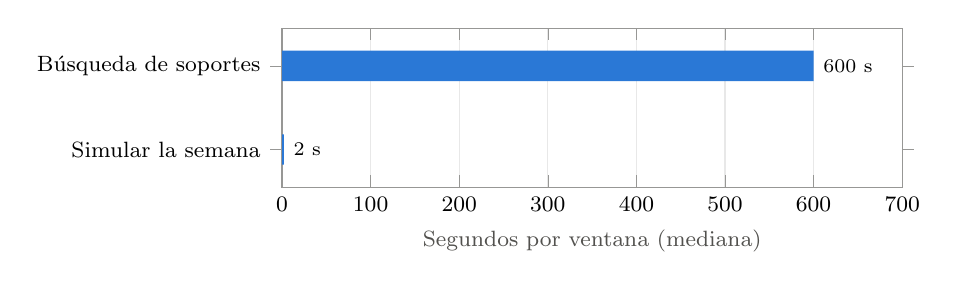
\begin{tikzpicture}
\begin{axis}[estilo, xbar, width=0.78\linewidth, height=3.6cm, bar width=11pt,
  y dir=reverse, ytick={1,2}, yticklabels={{Búsqueda de soportes}, {Simular la semana}},
  xmin=0, xmax=700, enlarge y limits=0.45, xlabel={Segundos por ventana (mediana)}, xmajorgrids,
  nodes near coords, every node near coord/.append style={font=\scriptsize, color=black},
  nodes near coords={\pgfmathprintnumber{\pgfplotspointmeta} s}, point meta=x]
\addplot[fill=serieA, draw=none] coordinates {(600,1) (2,2)};
\end{axis}
\end{tikzpicture}
\caption{Dónde se va el tiempo de una ventana. Lo que depende de \code{A}, \code{B} y
\code{PERDIDA\_MAX} cuesta 2 segundos; lo que no depende de ellos cuesta 600 y se repite en cada ventana.}
\label{fig:computo}
\end{figure}

\textbf{Por qué importa.} (1) Todo lo aprendido hasta ahora (\code{Q4} contra estática, la candidata, el
efecto de \code{A}) es sobre una estrategia de grilla\footnote{Grilla (\emph{grid trading}): poner órdenes
de compra a distancias iguales bajo el precio, sin elegir niveles. Aquí el paso de la grilla lo fija
\code{N}.} cuyo paso fija \code{N}, no sobre los soportes que elige X0. (2) Si la búsqueda no converge,
\code{K}, \code{N\_EXP} y \code{LAMBDA} no alcanzan a expresarse: no es casualidad que no muestren ninguna
señal. (3) Con cuenta nueva no hay órdenes abiertas en \code{t*}, así que los soportes de esa semana no
dependen de \code{A}, \code{B} ni \code{PERDIDA\_MAX}: probar 30 valores de \code{A} en la misma semana
podría costar 10 minutos más 30 $\times$ 2 segundos, no 300 minutos.

\textbf{Matiz.} Los archivos de producción que comparé son de septiembre, de una versión de X0 anterior a
los saltos del 3 de noviembre. La diferencia es demasiado grande para que eso la explique, pero hay que
confirmarlo (Sección~\ref{sec:propuesta}, pieza 2).

\textbf{Qué cambiaría.} Separar ``buscar soportes'' de ``operar'': reutilizar los soportes y simular cientos
de configuraciones de operación por semana. Y responder una pregunta que hoy nadie ha medido:
\emph{¿cuánto mejor que una grilla pareja es X0?}

% ────────────────────────────────────────────────────────────────────
\subsection{El diseño diluye la señal: 30 coeficientes en un modelo lineal}
\label{sec:ruido}

\textbf{Qué encontré.} Cinco mecanismos que se suman, y ningún modelo más sofisticado los arregla porque
son de diseño:
\begin{itemize}[leftmargin=1.2em]
  \item \textbf{El ruido de la semana.} En el mismo \code{t*}, la candidata y \code{Q4} se correlacionan
        0,94 (BTCUSD) y 0,97 (TSLA). Pero \code{ret\_medio} y \code{ret\_vol} explican solo el 14\% de $Y$ en
        validación cruzada\footnote{Validación cruzada: se ajusta el modelo con una parte de los datos y se
        mide su error en la que no vio. El $R^2$ (fracción de la variación explicada) medido así no se
        infla por sobreajuste; puede ser negativo si el modelo predice peor que el promedio.}. Lo que
        comparten las configuraciones no son dos números resumen: es el camino completo del precio. En TSLA
        la relación ni siquiera es lineal: por quintiles de \code{ret\_medio}, $Y$ medio es $-67$, 35, 56,
        57 y 35 (en las semanas de subida fuerte el precio se aleja de los soportes).
  \item \textbf{Un instrumento débil\footnote{Instrumento débil: se sortea limpiamente una variable (los C2)
        que empuja poco a la que de verdad actúa (los C1). El efecto llega tan diluido que el ruido lo
        tapa.}.} Los C2 explican solo entre el 8\% y el 43\% de la variación de los C1; el resto lo pone el
        estado del activo. Y regresar $Y$ sobre los C1 tampoco sirve, porque los C1 dependen del estado y el
        estado mueve $Y$ (confusión\footnote{Confusión (\emph{confounding}): una tercera variable mueve a la
        vez la causa supuesta y el resultado, y crea o tapa una relación aparente.}).
  \item \textbf{Efectos que se cancelan.} La derivada de un C1 respecto de su pendiente tiene el signo de
        $s_t - \text{punto\_medio}$, que cambia de ventana en ventana. Un modelo lineal promedia efectos de
        signo opuesto: para \code{p}, el signo medio es $-0{,}08$; aunque la pendiente importara mucho, su
        coeficiente saldría cerca de cero.
  \item \textbf{Saturación.} Las pendientes llegan a 8--12: \code{K} funciona como un interruptor, pegado al
        10\% extremo de su rango en el 63\% de las ventanas de BTCUSD, donde mover los C2 no cambia nada.
  \item \textbf{Un ascenso que camina haya señal o no.} El C2 de mayor efecto se mueve siempre el 10\% de
        su rango (\code{x5\_alt\_aprendizaje.py:205-207}), aunque la regresión esté encogiendo todo al
        máximo (ridge en el tope de su grilla en 27 de las primeras 40 propuestas de BTCUSD y en el 64\% de
        las de TSLA). Después del Sobol no hay exploración y los signos están fijados a mano: el
        aprendizaje no puede descubrir que una hipótesis está al revés.
\end{itemize}

Con ese ruido, la estadística es implacable. Para detectar una mejora con una potencia
estadística\footnote{Potencia: probabilidad de detectar un efecto que sí existe. Lo usual es exigir 80\%.}
de 80\% se necesitan $n \approx (2{,}8\,\sigma/\delta)^2$ semanas, con $\sigma$ la desviación de la
diferencia pareada (Tabla~\ref{tab:potencia}). En BTCUSD se suman colas muy pesadas: el 5\% de las semanas
aporta el 60\% de la suma de $Y$ (curtosis\footnote{Curtosis: cuán frecuentes son los valores extremos.
Una distribución normal tiene 0 (en exceso); $Y$ de BTCUSD tiene 26.} de 26), y la RLM ajusta promedios,
justo el estadístico que dominan esas pocas semanas.

\begin{table}[h]
\centering\small
\begin{tabular}{lcccc}
\toprule
Efecto a detectar & BTCUSD pareado & BTCUSD sin parear & TSLA pareado & TSLA sin parear \\
\midrule
10 USD/semana & 7.491 & 30.693 & 443 & 1.352 \\
25 USD/semana & 1.199 & 4.911 & 71 & 217 \\
50 USD/semana & 300 & 1.228 & 18 & 55 \\
\bottomrule
\end{tabular}
\caption{Semanas necesarias para detectar una mejora media (80\% de potencia, 5\% de significancia).
Historia disponible: unas 240 semanas por valor.}
\label{tab:potencia}
\end{table}

El resultado ya lo viste el 21 de noviembre: los C2 no explican $Y$ por sobre el mercado. Agrego que
tampoco los siete C1 realizados lo explican ($R^2$ fuera de pliegue de $-0{,}03$ y $-0{,}11$). No es un
problema de modelo; es de diseño y de resolución.

\textbf{Qué cambiaría.} Dejar de aprender C2. Sortear los C1 directamente, \emph{dentro de la misma
semana}, y restar el mercado completo comparando en pares.

% ────────────────────────────────────────────────────────────────────
\subsection{La ventana semanal ve la mitad buena de la estrategia}
\label{sec:mitad}

\textbf{Qué encontré.} La estrategia gana poco y seguido (trailing stop) y pierde mucho y junto (pérdida
máxima). En una semana con cuenta nueva solo se alcanza a ver lo primero: gana el 98,8\% de los trades
cerrados de BTCUSD, el 27--33\% de las posiciones sigue abierta al cierre y las pérdidas quedan como
flotante (suma de lo cerrado +37.151 USD, de lo abierto $-17.589$). La cuenta continua cuenta otra
historia (Figura~\ref{fig:continua}).

\begin{figure}[h]
\centering
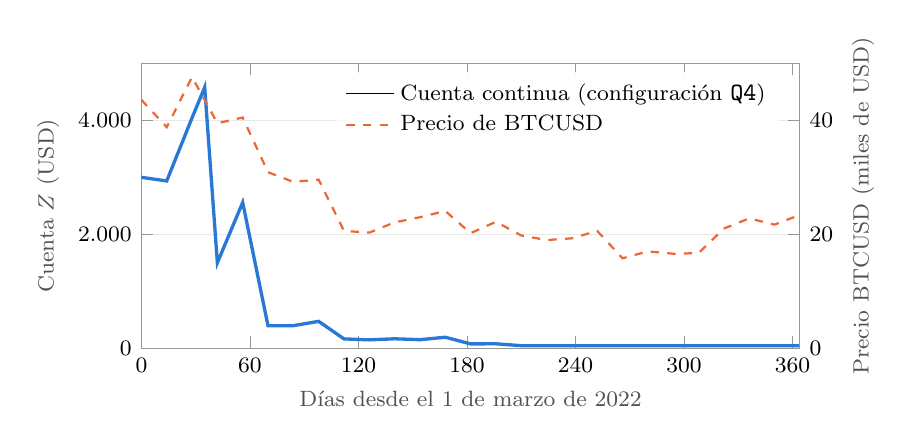
\begin{tikzpicture}
\begin{axis}[estilo, width=0.82\linewidth, height=5.2cm, xmin=0, xmax=364, ymin=0, ymax=5000,
  xlabel={Días desde el 1 de marzo de 2022}, ylabel={Cuenta $Z$ (USD)}, axis y line*=left, ymajorgrids,
  xtick={0,60,120,180,240,300,360}]
\addplot[serieA, very thick, mark=none] coordinates {(0,3000) (14,2937) (28,4043) (35,4581) (42,1501) (56,2559) (70,396) (84,397) (98,473) (112,165) (126,148) (140,167) (154,151) (168,194) (182,77) (196,79) (210,46) (224,46) (238,46) (252,46) (266,46) (280,46) (294,46) (308,46) (322,46) (336,46) (350,46) (364,46)};
\label{pl:z}
\end{axis}
\begin{axis}[estilo, width=0.82\linewidth, height=5.2cm, xmin=0, xmax=364, ymin=0, ymax=50,
  axis y line*=right, axis x line=none, ylabel={Precio BTCUSD (miles de USD)},
  legend style={at={(0.97,0.97)}, anchor=north east, fill=white, fill opacity=0.9, text opacity=1}]
\addlegendimage{/pgfplots/refstyle=pl:z}\addlegendentry{Cuenta continua (configuración \code{Q4})}
\addplot[serieB, thick, dashed, mark=none] coordinates {(0,43.6) (14,38.8) (28,47.6) (42,39.5) (56,40.5) (70,30.9) (84,29.2) (98,29.6) (112,20.6) (126,20.3) (140,22.1) (154,23.0) (168,24.1) (182,20.2) (196,22.2) (210,19.8) (224,19.0) (238,19.3) (252,20.6) (266,15.8) (280,17.0) (294,16.6) (308,16.7) (322,21.0) (336,22.8) (350,21.7) (364,23.4)};
\addlegendentry{Precio de BTCUSD}
\end{axis}
\end{tikzpicture}
\caption{Cuenta continua \code{q4\_s0\_v2} (\code{BTCUSD\_seguimiento.csv}). Subió a 4.581 USD y cayó a
396 entre el 5 de abril y el 10 de mayo de 2022; terminó en 46 y no volvió a operar. El 27\% de sus cierres
fue por pérdida máxima (233 de 870, $-30{,}5$ USD en promedio) contra 637 por trailing stop ($+6{,}5$).}
\label{fig:continua}
\end{figure}

Hay que decir el límite de la comparación: esa cuenta corrió antes del tope de Órdenes Abiertas (OA) y con
un umbral de pérdida que se achicaba con la cuenta, lo que creó una espiral. El tope actual la limita, pero
no cambia el fondo: \textbf{el riesgo de esta estrategia vive en secuencias de semanas} (pérdidas
correlacionadas que se acumulan y ocupan el cupo de OA), y una ventana que parte limpia cada lunes no las
ve. Un dato lo ilustra: la estática promedia +145 USD por semana en las ventanas de BTCUSD sobre 3.000 USD,
unas 2,5 veces la cuenta al año. Nadie ha verificado que una cuenta continua con la estática se acerque.

Tres sesgos más empujan en la misma dirección. (1) $Y$ sube con el número de trades (correlación 0,65 en
BTCUSD): la semana premia rotar rápido, y eso hace la estática con \code{A = 3}. (2) El backtest no cobra
spread\footnote{Spread: diferencia entre el precio de compra (Ask) y el de venta (Bid). Las velas de
MetaTrader son de Bid; una compra límite se ejecuta cuando el Ask, un spread más arriba, llega al precio.}:
la orden se llena apenas el mínimo de la vela toca el soporte (\code{X4\_backtester.py:507}). Lo estimé con
la columna \code{Spread} de los datos: 9\% de la suma de $Y$ en BTCUSD y 4\% en TSLA; no cambia ninguna
conclusión, pero favorece a quien opera más. El financiamiento nocturno (swap) no lo pude estimar. (3) La
compuerta usa la mediana, que es ciega justo a las semanas que quiebran la cuenta.

\textbf{Qué cambiaría.} Usar la ventana para \emph{explorar} (es barata y pareable), medir el destino de
las posiciones abiertas (seguir gestionándolas sin abrir nuevas hasta que cierren: segundos de cómputo) y
\emph{decidir} con una cuenta continua y una medida de la cola izquierda, como el CVaR\footnote{CVaR
(\emph{Conditional Value at Risk}) al 10\%: el promedio del 10\% de peores semanas. Una regla como ``CVaR
no peor que $-300$ USD'' acota cuánto se pierde en las semanas malas.}.

% ────────────────────────────────────────────────────────────────────
\subsection{Se compara nivel, no dinamismo, y el ancla fue Q4}
\label{sec:ancla}

\textbf{Qué encontré.} \code{Q4} calibró cada curva contra un objetivo de diseño (su propio percentil), sin
resultado económico detrás; la revisión de octubre ya mostró que ese ajuste no puede fallar. En las
ventanas pierde contra la estática con significancia, en ambos valores y en todos los años:

\begin{table}[h]
\centering\small
\begin{tabular}{lccccc}
\toprule
Suma de $Y$ en \code{t*} reservados & 2022 & 2023 & 2024 & 2025 & 2026 \\
\midrule
BTCUSD estática / \code{Q4} & $-174$ / $-771$ & 207 / 154 & 697 / $-126$ & 4.724 / 2.740 & 713 / 344 \\
TSLA estática / \code{Q4} & 504 / $-294$ & 264 / $-44$ & 490 / 36 & 911 / 235 & 279 / 97 \\
\bottomrule
\end{tabular}
\caption{La estática le gana a \code{Q4} en 10 de 10 años-valor.}
\end{table}

Pierde sobre todo por \emph{nivel}. \code{Q4} opera en promedio con \code{A} $\approx$ 8,8 USD (BTCUSD) y
7,5 (TSLA); la estática con 3. Con \code{A} más alto se abren menos órdenes (correlación de rangos entre
\code{A} y trades de $-0{,}32$ y $-0{,}64$) y en TSLA el resultado cae ordenadamente con \code{A}
(Figura~\ref{fig:A}). El aprendizaje partió de \code{Q4} y caminó de vuelta hacia la estática: la
candidata de BTCUSD terminó en \code{A} $\approx$ 6. Unas 130 ventanas (22 horas de cómputo) para
redescubrir a medias que \code{A} bajo opera más.

\begin{figure}[h]
\centering
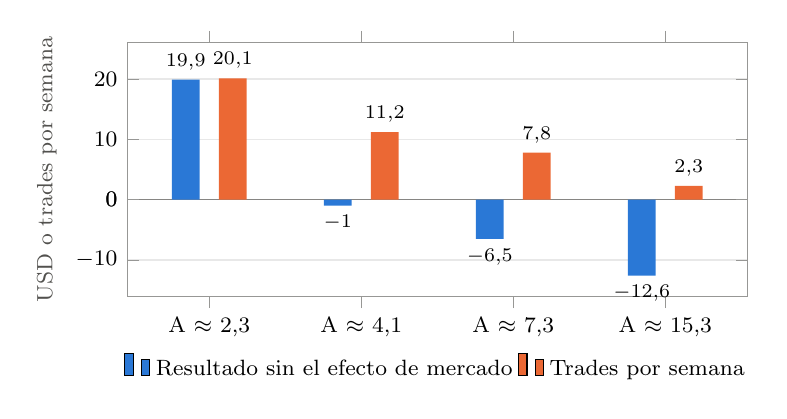
\begin{tikzpicture}
\begin{axis}[estilo, ybar=7pt, width=0.78\linewidth, height=4.8cm, bar width=10pt,
  symbolic x coords={q1,q2,q3,q4}, xtick=data,
  xticklabels={{A $\approx$ 2,3}, {A $\approx$ 4,1}, {A $\approx$ 7,3}, {A $\approx$ 15,3}},
  ymin=-16, ymax=26, ymajorgrids, ylabel={USD o trades por semana},
  extra y ticks={0}, extra y tick style={grid=major, major grid style={tinta2!70}},
  enlarge x limits=0.18, legend style={at={(0.5,-0.2)}, anchor=north}, legend columns=2,
  nodes near coords, every node near coord/.append style={font=\scriptsize, color=black},
  nodes near coords={\pgfmathprintnumber[fixed, precision=1]{\pgfplotspointmeta}}]
\addplot[fill=serieA, draw=none] coordinates {(q1,19.9) (q2,-1.0) (q3,-6.5) (q4,-12.6)};
\addplot[fill=serieB, draw=none] coordinates {(q1,20.1) (q2,11.2) (q3,7.8) (q4,2.3)};
\legend{Resultado sin el efecto de mercado\quad, Trades por semana}
\end{axis}
\end{tikzpicture}
\caption{TSLA, ventanas de aprendizaje agrupadas por cuartil de \code{A}. A menor \code{A}, más trades y
mejor resultado, con el mejor grupo en el piso del rango actual. En BTCUSD la relación no es ordenada (el
mejor cuartil está en \code{A} $\approx$ 5,8).}
\label{fig:A}
\end{figure}

\textbf{Por qué importa.} Comparar ``dinámico contra estático'' con niveles medios tan distintos mide el
nivel, no el dinamismo (la revisión de octubre lo advirtió para \code{N}; hoy pesa más en \code{A}). Y la
forma de la curva mezcla ambos: con punto medio y pendiente no hay forma simple de decir ``la estática,
más una pequeña modulación''.

\textbf{Qué cambiaría.} Primero buscar el mejor nivel estático. Después, si se justifica, una dinámica
anclada en ese nivel: $C1_t = C1^{*} \cdot e^{\beta\, s_t}$ (recortado a piso y techo), donde $\beta = 0$ es
exactamente la estática. Dos números con significado claro (nivel y sensibilidad) en vez de cuatro o cinco.

% ────────────────────────────────────────────────────────────────────
\subsection{Una compuerta que deja pasar ruido}
\label{sec:compuerta}

\textbf{Qué encontré.} La candidata se promueve si la mediana de su diferencia contra la estática y contra
\code{Q4} es positiva, sin medir incertidumbre. Si la candidata fuera en realidad igual a la estática, ese
criterio se pasaría la mitad de las veces por azar; y como \code{Q4} es un rival débil, exigir ganarle
también casi no filtra.

\begin{table}[h]
\centering\small
\begin{tabular}{lccccc}
\toprule
Comparación (mismo \code{t*}) & $n$ & Media (IC 95\%) & Mediana (IC 95\%) & Gana & p \\
\midrule
BTCUSD candidata $-$ estática & 26 & $-34$ ($-214$; 114) & 14 ($-24$; 63) & 15/26 & 0,56 \\
BTCUSD candidata $-$ \code{Q4} & 26 & 62 (25; 98) & 43 (8; 116) & 21/26 & 0,002 \\
BTCUSD \code{Q4} $-$ estática & 44 & $-87$ ($-184$; $-4$) & $-31$ ($-60$; $-13$) & 11/44 & 0,001 \\
TSLA candidata $-$ estática & 24 & $-55$ ($-81$; $-32$) & $-45$ ($-71$; $-17$) & 4/24 & 0,002 \\
TSLA candidata $-$ \code{Q4} & 24 & 18 (10; 26) & 11 (4; 30) & 20/24 & 0,002 \\
TSLA \code{Q4} $-$ estática & 47 & $-52$ ($-73$; $-32$) & $-26$ ($-51$; $-14$) & 11/47 & $<$0,001 \\
\bottomrule
\end{tabular}
\caption{Diferencias de $Y$ (USD por semana). Intervalos de confianza por remuestreo\protect\footnotemark;
p de la prueba de signo\protect\footnotemark.}
\label{tab:compuerta}
\end{table}
\footnotetext[\the\numexpr\value{footnote}-1\relax]{Intervalo de confianza (IC) por remuestreo
(\emph{bootstrap}): se sortean muchas veces, con reemplazo, las semanas observadas y se recalcula el
estadístico; el IC 95\% es el rango donde cae el 95\% central de esos recálculos. Si incluye el cero, no se
puede descartar que no haya diferencia.}
\footnotetext{Prueba de signo: si dos configuraciones fueran igual de buenas, cada una ganaría la mitad
de las semanas. El valor p es la probabilidad de ver un resultado tan desbalanceado o más solo por azar.}

\textbf{Lectura.} El aprendizaje sí aprende algo: mejora sobre \code{Q4} con claridad. Pero no supera a la
estática. En BTCUSD la promoción descansa en una mediana de +14 USD cuyo intervalo incluye el cero, con
media negativa: es indistinguible del azar. Con 26 semanas, la compuerta solo puede ver mejoras de unos 240
USD por semana en BTCUSD, seis veces la ganancia media de la estrategia. Y cada candidata nueva evaluada
contra las mismas semanas reservadas es otro boleto de lotería (la ``maldición del
ganador''\footnote{Maldición del ganador: si se prueban muchas candidatas y se queda la que mejor salió, su
resultado medido está inflado por la suerte y en datos nuevos rinde menos.}).

\textbf{Qué cambiaría.} Promover solo si el límite inferior del intervalo de la mejora media es positivo en
un período de prueba posterior al de entrenamiento, contra la \emph{mejor estática} (no \code{Q4}), con el
CVaR no peor y la cuenta continua sin empeorar la caída máxima. La candidata que hoy está en la demo sirve
para probar la mecánica, no como evidencia de mejora; eso ya lo dejaste anotado.

% ════════════════════════════════════════════════════════════════════
\section{La revisión de octubre, un mes después}

La revisión del 23 de octubre se hizo antes del cambio a ventanas semanales. Qué pasó con sus hallazgos:

\begin{table}[h]
\centering\small
\begin{tabularx}{\linewidth}{@{}>{\raggedright\arraybackslash}p{5.4cm}>{\raggedright\arraybackslash}p{2.2cm}>{\raggedright\arraybackslash}X@{}}
\toprule
Hallazgo de octubre & Estado & Por qué \\
\midrule
La evidencia ``alta'' de \code{Q3} era mecánica & Vigente & Los signos de cada variable siguen saliendo de
ahí y el aprendizaje no los puede invertir. \\
La calibración de \code{Q4} no puede fallar & Vigente & Se sortea ``cerca de \code{Q4}'' y \code{Q4} pierde en
todos los años. \\
El \code{N} dinámico es sobre todo un \code{N} más bajo & Vigente y agravado & Ahora pesa más en \code{A}
(8,8 contra 3). \\
Objetivo ajustado por riesgo & Parcial & El tope de OA controla el riesgo de la cuenta, pero $Y$ y la compuerta
siguen sin mirar la cola izquierda. \\
\code{A}, \code{B} y \code{PERDIDA\_MAX} en dólares & Vigente & Un mismo \code{A} en USD significa cosas
distintas con BTC a 16 mil o a 100 mil. \\
\code{K}, \code{N\_EXP} y \code{LAMBDA} no deberían ser dinámicos & Vigente y agravado & Hoy se publican así
en la demo. \\
$\mu$ y $\sigma$ con información del futuro & Resuelto & Ventana expansiva. \\
Fundamentales de X2 & Resuelto & Fuera del modelo. \\
Piloto chico con estáticos de distinto nivel & No se hizo & Hoy es barato: es casi la pieza 4 de la propuesta. \\
\bottomrule
\end{tabularx}
\caption{Estado de la revisión del 23 de octubre (\code{x5\_alt\_v2\_opus.pdf}).}
\end{table}

La lección que deja la tabla: varias advertencias de octubre se cumplieron porque se avanzó a construir
la siguiente capa antes de probar la anterior. La propuesta de este informe está ordenada para que eso no
vuelva a pasar: cada pieza tiene una prueba que la puede tumbar antes de construir encima.

% ════════════════════════════════════════════════════════════════════
\section{Tus cuatro ideas}
\label{sec:ideas}

\subsection*{1. Estudiar los C1 de a uno — sí, con condiciones}
A favor: baja las dimensiones de 30 a 1--3, aísla causas y permite cerrar cada C1 con un sí o un no. En
contra: mover un factor a la vez pierde interacciones (por ejemplo, \code{A} con la pérdida máxima) y es
ineficiente cuando probar es barato. Por eso: los tres de \textbf{operación} (\code{A}, \code{factor\_B},
\code{p}) se estudian \emph{juntos} en una grilla, porque reutilizando soportes cuestan segundos; los cuatro
de \textbf{búsqueda} (\code{N}, \code{K}, \code{N\_EXP}, \code{LAMBDA}) sí van de a uno, o se fijan. Y cada
C1 responde dos preguntas en orden: primero cuál es su mejor nivel estático; después, si moverlo agrega algo
sobre ese nivel.

\subsection*{2. Construir desde todo el universo de variables — sí, contra un objetivo limpio}
Con 240 semanas y 50 variables candidatas contra $Y$ semanal, la mejor saldrá ``buena'' por puro azar. La
idea funciona si se cambia la pregunta. En vez de ``¿esta variable explica $Y$?'', preguntar: ``¿cuando
esta variable está alta, convenía un \code{A} más alto?''. El objetivo es
$u_w = Y_w(\text{A alto}) - Y_w(\text{A bajo})$, en la misma semana, con los mismos soportes y la misma
semilla: el mercado se cancela dentro del par. Protocolo:
\begin{enumerate}[leftmargin=1.4em]
  \item Agrupar candidatas por familia (volatilidad, tendencia, drawdowns de 7/30/90 días, rango, volumen,
        sentimiento, Fibonacci) y dejar una por grupo de variables muy correlacionadas: 10 a 20.
  \item Validar por bloques de tiempo contiguos, nunca con semanas al azar\footnote{Validación por bloques
        (\emph{blocked} o \emph{purged cross-validation}): los pliegues son trimestres seguidos, con una semana
        de separación a cada lado, para que el modelo no aprenda de semanas vecinas a las que evalúa.}.
  \item Corregir por haber probado muchas: barajar $u_w$ y ver qué tan buena sale la \emph{mejor} variable
        por azar (permutación del máximo), o controlar la tasa de falsos descubrimientos\footnote{Tasa de
        falsos descubrimientos (FDR, \emph{False Discovery Rate}, método de Benjamini-Hochberg): con 100
        variables, unas 5 parecerán útiles por azar; el método ajusta el umbral para acotar la fracción de
        falsas entre las declaradas útiles.}.
  \item Exigir estabilidad: mismo signo en al menos 4 de 5 años y en BTCUSD y TSLA.
  \item Pre-registrar como máximo 1--2 variables por C1, con su signo, antes de confirmarlas.
\end{enumerate}
Los fundamentales de X2 quedan fuera: su historial solo cubre junio a septiembre de 2026, y usarlos hacia
atrás metería información del futuro. Fear \& Greed sí se puede reconstruir.

\subsection*{3. Una red neuronal (FFNN) en vez de la RLM — no ahora}
Con unas 120 ventanas útiles, una Red Neuronal de Alimentación Hacia Adelante (FFNN) con 26 entradas y 16
neuronas ocultas tiene 449 parámetros: sobreajusta, y no arregla ni el instrumento débil ni la cancelación
de signos, que son de diseño. Cambia todo cuando existan los datos de la grilla: unas 240 semanas por 50
configuraciones son 12.000 filas para un modelo sustituto $Y \approx g(\text{C1}, \text{estado})$. Aun ahí,
en datos tabulares lo primero es Gradient Boosting (GB) con restricciones de monotonía\footnote{Restricción
de monotonía: obligar al modelo a que, por ejemplo, más volatilidad nunca baje \code{A}. Le da el ``sentido
lógico'' que pides y reduce el sobreajuste.} o un Modelo Aditivo Generalizado (GAM): rinden igual o mejor y
se pueden leer. La FFNN entra si les gana en validación por bloques. Para los parámetros caros (los de
búsqueda, 1 a 3 dimensiones), la herramienta correcta es la optimización bayesiana (BO) con proceso
gaussiano (GP)\footnote{Optimización bayesiana con proceso gaussiano: un método para optimizar funciones
caras y ruidosas con pocas evaluaciones; elige el próximo punto a probar balanceando ``donde creo que es
bueno'' con ``donde todavía sé poco''.}.

\subsection*{4. Mantener C1 = f(C2) con evolución lógica en el tiempo — sí, reformulada}
La misión queda como $C1_t = \pi(\text{estado}_t)$: una regla de pocas dimensiones, monótona (el sentido
lógico como restricción o, mejor, como algo que se prueba), con histéresis\footnote{Histéresis: cambiar de
régimen solo si el nuevo estado se sostiene un tiempo (por ejemplo, 24 horas), para que el parámetro no
salte de ida y vuelta por ruido.}, reestimada una vez al mes con la historia acumulada y validada hacia
adelante. ``Evolucionar en el tiempo'' significa eso: la regla se recalibra cuando llegan semanas nuevas.
La condición dura: un C1 solo se vuelve dinámico si pasa la prueba de que su mejor valor cambia con el
estado. Si no cambia, la mejor política es constante, y un C1 dinámico solo agrega ruido y rotación de
órdenes. Llegar a ``mejor estática, en unidades de volatilidad, más el tope de OA'' sería un éxito, no un
fracaso.

% ════════════════════════════════════════════════════════════════════
\section{Propuesta X5\_v3}
\label{sec:propuesta}

La idea central: \textbf{medir bien, después aprender, y de a poco}. Ocho piezas, en orden de valor sobre
esfuerzo. La versión con archivos, costos y criterios está en \code{X5\_v3.md} §8.

\begin{figure}[h]
\centering
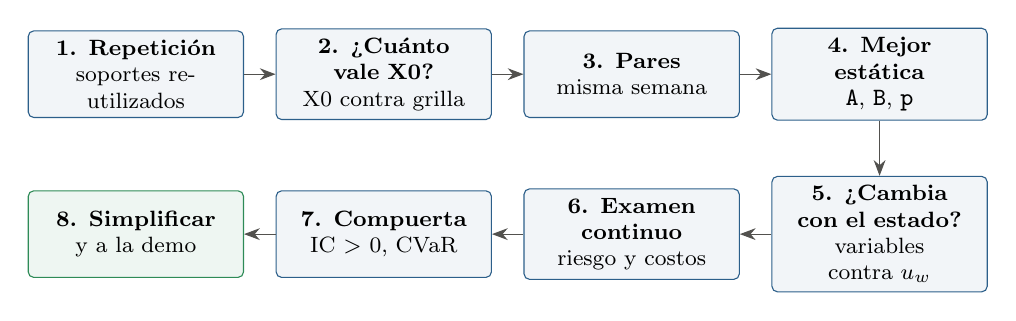
\begin{tikzpicture}[node distance=4mm and 4mm, every node/.style={font=\footnotesize, align=center},
  caja/.style={draw=cazul, rounded corners=2pt, fill=cazul!6, minimum height=11mm, text width=25mm},
  flecha/.style={-{Stealth[length=2mm]}, draw=tinta2}]
\node[caja] (r) {\textbf{1. Repetición}\\soportes reutilizados};
\node[caja, right=of r] (x) {\textbf{2. ¿Cuánto vale X0?}\\X0 contra grilla};
\node[caja, right=of x] (p) {\textbf{3. Pares}\\misma semana};
\node[caja, right=of p] (e) {\textbf{4. Mejor estática}\\\code{A}, \code{B}, \code{p}};
\node[caja, below=7mm of e] (h) {\textbf{5. ¿Cambia con el estado?}\\variables contra $u_w$};
\node[caja, left=of h] (c) {\textbf{6. Examen continuo}\\riesgo y costos};
\node[caja, left=of c] (k) {\textbf{7. Compuerta}\\IC $>$ 0, CVaR};
\node[caja, left=of k, fill=cverde!8, draw=cverde] (d) {\textbf{8. Simplificar}\\y a la demo};
\draw[flecha] (r) -- (x); \draw[flecha] (x) -- (p); \draw[flecha] (p) -- (e);
\draw[flecha] (e) -- (h); \draw[flecha] (h) -- (c); \draw[flecha] (c) -- (k); \draw[flecha] (k) -- (d);
\end{tikzpicture}
\caption{Orden propuesto. Las piezas 1 a 3 arreglan el instrumento; 4 y 5 aprenden; 6 a 8 deciden.}
\label{fig:flujo}
\end{figure}

\textbf{1. Motor de repetición.} Separar ``buscar'' de ``operar'' en \code{ejecutar\_ventana}: copiar el
estado tras la búsqueda y simular la semana con muchas combinaciones de (\code{A}, \code{factor\_B},
\code{p}), con la misma semilla. Se puede empezar \emph{hoy} con los 562 juegos de soportes que ya están
guardados, sin búsquedas nuevas. \emph{Valida}: repetir 20 ventanas con su propia configuración reproduce
$Y$ al centavo. \emph{Costo}: 2--4 horas de desarrollo; después, 2 segundos por configuración y semana.

\textbf{2. ¿Cuánto vale X0?} En 20 a 40 semanas, buscar soportes como en producción (partiendo de la
solución de la semana anterior, 30--60 minutos) y comparar contra la grilla pareja actual, con la estática.
Si X0 rinde igual que la grilla, la estrategia es en el fondo una grilla y el sistema se simplifica mucho
(\code{N} pasa a ser el paso). Si X0 rinde más, hace falta un banco de soportes de calidad producción
(unas 40 horas por valor, una sola vez) antes de estudiar los parámetros de búsqueda. Cualquiera de los dos
resultados vale. \emph{Costo}: 10--20 horas de cómputo.

\textbf{3. Pares por semana y ruido medido.} Toda configuración se evalúa en las mismas semanas que una
referencia y la métrica es $D_w = Y_w(\theta) - Y_w(\text{ref})$: un efecto fijo por
semana\footnote{Efecto fijo por semana: en vez de explicar qué tuvo de especial cada semana con unas pocas
variables, se compara todo dentro de la misma semana, de modo que lo especial se cancela en la resta.}.
Intervalos por remuestreo de bloques de semanas. \code{ret\_medio} y \code{ret\_vol} salen del modelo. Y
medir por fin el ruido: misma configuración con dos semillas de la simulación dentro de la vela.

\textbf{4. Mejor estática.} Grilla de los tres de operación: \code{A} en \{1; 1,5; 2; 3; 4; 6; 8; 12\} USD
y también en unidades de volatilidad ($A_t = k_A \cdot \text{ATR}_t$, con ATR\footnote{Rango verdadero
promedio (ATR, \emph{Average True Range}): tamaño típico del movimiento de una vela, en unidades de precio.
Expresar \code{A} así lo adapta solo al activo y al régimen, con un único número.} el movimiento típico de
una vela), \code{factor\_B} en \{0,3; 0,5; 0,7\} y \code{p} en \{0,03; 0,045; 0,067; 0,09\}. Elegir con datos
hasta junio de 2024 y medir después (validación hacia adelante\footnote{Validación hacia adelante
(\emph{walk-forward}): elegir con el pasado y medir en un período posterior que no se usó para elegir.}),
prefiriendo una meseta (una zona donde los vecinos también rinden) antes que el pico. \emph{Costo}: unas
13 horas por valor.

\textbf{5. ¿El mejor valor cambia con el estado?} Con la grilla, aplicar el protocolo de la idea 2 a
\code{A} y \code{p}. Solo si una variable pasa, el C1 se vuelve dinámico, con la forma más simple que
alcance: anclada en la estática ($C1^{*}e^{\beta s_t}$) o una tabla de 2--3 regímenes con histéresis.
\emph{Costo}: minutos.

\textbf{6. Examen continuo, con costos.} Antes de promover, correr candidata y estática en una cuenta
continua 2022--2026 (minutos, con los soportes reutilizados), con valor final, caída máxima, CVaR y razón
de Calmar\footnote{Razón de Calmar: retorno anual dividido por la caída máxima de la cuenta. Premia ganar
sin pasar por pozos profundos.}. Cobrar el spread en \code{X4\_backtester.py} y medir el swap con los deals
que ya guarda \code{registro\_din.py}. Registrar también el resultado de las posiciones abiertas llevadas a
su cierre.

\textbf{7. Compuerta nueva.} La de la sección~\ref{sec:compuerta}. Se valida con un candidato nulo (la
estática contra sí misma con otra semilla): debe pasar menos del 10\% de las veces; la regla actual pasa
cerca del 50\%. \emph{Costo}: 1--2 horas.

\textbf{8. Simplificar.} Fijar \code{K}, \code{N\_EXP} y \code{LAMBDA} por valor (hoy se publican como
dinámicos en la demo sin evidencia, y cambian lo que X0 optimiza en vivo) y buscar \code{N} solo por
nivel. Recalibrar la regla una vez al mes.

\begin{clave}
\textbf{Cómo se vería la solución final (hipótesis a confirmar).} Por valor: \code{N}, \code{K},
\code{N\_EXP} y \code{LAMBDA} fijos; \code{A} en unidades de volatilidad, quizás modulado por una variable
si pasa la prueba de la pieza 5; \code{B} = \code{factor\_B} $\cdot$ \code{A}; pérdida máxima y tope de OA
como política de riesgo. Entre 6 y 10 números por valor, cada uno con evidencia, recalibrados una vez al
mes. Simple de entender, barato de recalcular y fácil de auditar.
\end{clave}

% ════════════════════════════════════════════════════════════════════
\section{Plan de pruebas para las próximas 2 a 4 semanas}
\label{sec:plan}

Cada fase lleva su criterio de éxito escrito \emph{antes} de correrla (pre-registro en
\code{decisiones.md}), para no mover la vara después de ver el resultado.

\begin{table}[h]
\centering\small
\begin{tabularx}{\linewidth}{@{}>{\raggedright\arraybackslash}p{2.1cm}>{\raggedright\arraybackslash}X>{\raggedright\arraybackslash}X>{\raggedright\arraybackslash}p{1.4cm}@{}}
\toprule
Fase & Qué se hace & Criterio pre-registrado & Cómputo \\
\midrule
0. Reglas (días 1--2) & Pausar la fase RLM. Compuerta nueva. Reservar un bloque final de semanas que no se
mira hasta la fase 4. & Un candidato nulo pasa la compuerta menos del 10\% de las veces. & — \\
1. Instrumento (semana 1) & Motor de repetición. Ruido de la simulación (2 semillas, 20 semanas) y de la
búsqueda (10 semanas). Spread en X4. & Reproduce $Y$ al centavo. Si el ruido de la búsqueda supera la mitad
de la diferencia entre configuraciones, la fase 2 va primero. & 2 h \\
2. ¿Cuánto vale X0? (semanas 1--2) & 20--40 semanas con búsqueda tipo producción contra la grilla actual.
& Decide si hace falta un banco de soportes de calidad producción antes de seguir con \code{N}. & 10--20 h \\
3. Mejor estática (semana 2) & Grilla de \code{A} (USD y ATR), \code{factor\_B} y \code{p}, en pares.
Cuenta continua de la estática actual y de la mejor. & Se adopta si la media pareada tiene IC 90\% sobre 0
en el período de prueba, el CVaR no empeora más de 10\% y la cuenta continua no empeora la caída máxima. &
6--15 h \\
4. ¿Dinamismo? (semanas 3--4) & Protocolo de la idea 2 para \code{A} y \code{p}; una sola evaluación en el
bloque reservado; demo. & Pasa permutación del máximo (p $\leq$ 0,05) y mismo signo en BTCUSD y TSLA. Si
no, el C1 queda estático. & minutos \\
\bottomrule
\end{tabularx}
\caption{Plan por fases. Lo que pase la fase 3 o la 4 reemplaza a la candidata actual en la demo.}
\label{tab:plan}
\end{table}

\textbf{Regla de cierre}: si ni \code{A} ni \code{p} muestran que su mejor valor cambia con el estado, esta
etapa se cierra como ``mejor estática (en unidades de volatilidad si gana) más tope de OA''. Es una
entrega útil, simple y, sobre todo, respaldada. Cómputo total: 25 a 45 horas por valor, contra unas 46
horas por valor para 250 ventanas del diseño actual, cada una con una sola configuración.

% ════════════════════════════════════════════════════════════════════
\section{Decisiones que te tocan}

Antes de construir nada, estas decisiones son tuyas. Para cada una, lo que recomiendo:

\begin{enumerate}[leftmargin=1.4em]
  \item \textbf{¿Pausar el orquestador actual y la fase RLM?} Recomiendo sí: hoy cada ventana cuesta 10
        minutos y no mueve nada.
  \item \textbf{¿Volver \code{K}, \code{N\_EXP} y \code{LAMBDA} a estáticos en la demo?} Recomiendo sí,
        hasta que la pieza 2 diga si importan.
  \item \textbf{¿Qué riesgo aceptas?} El objetivo pasa a ser ``ganar más, sujeto a un límite de pérdida en
        las peores semanas y en la cuenta continua''. El número lo pones tú; propongo partir con un CVaR al
        10\% no peor que el de la estática actual (hoy $-300$ USD por semana en BTCUSD y $-85$ en TSLA) y una
        caída máxima de la cuenta continua bajo 40\%.
  \item \textbf{¿Cobrar el spread en X4?} Recomiendo sí, con una opción para apagarlo y comparar contra
        resultados anteriores. Cambia todos los backtests, no solo los de X5.
  \item \textbf{¿Qué semanas quedan intocables?} Recomiendo reservar las últimas 26 semanas de la historia
        (desde mayo de 2026) para una única confirmación en la fase 4, más la demo hacia adelante.
  \item \textbf{¿Aceptas que el resultado pueda ser ``mejor estática más tope de OA''?} Es la pregunta de
        fondo. Si la respuesta es sí, el plan se puede correr sin sesgo; si la respuesta es ``tiene que salir
        algo dinámico'', el riesgo es volver a encontrar lo que se busca.
\end{enumerate}

% ════════════════════════════════════════════════════════════════════
\section{Qué dejaría de hacer ya}

\begin{itemize}[leftmargin=1.2em]
  \item \textbf{Correr más ventanas del esquema actual.} Cada una cuesta 10 minutos y entra a una regresión
        sin señal; además, el 26\% de las corridas ya se descarta por solaparse con una reservada.
  \item \textbf{Agregar variables a la RLM actual} o pasar a una red neuronal: el cuello de botella es la
        señal, no la capacidad del modelo.
  \item \textbf{Publicar \code{K}, \code{N\_EXP} y \code{LAMBDA} dinámicos en la demo}: cambian lo que X0
        optimiza en vivo sin ninguna evidencia a favor.
  \item \textbf{Leer la demo como evidencia de rendimiento}: unas semanas de demo son ruido, por las mismas
        razones de la Tabla~\ref{tab:potencia}. Sirve para validar la mecánica.
  \item \textbf{Plata real} antes de que una configuración pase la fase 3 y la cuenta continua.
\end{itemize}

\begin{clave}
\textbf{En una frase}: el proyecto no está estancado por falta de ideas ni de modelos, sino porque el
instrumento de medición no tiene la resolución para la pregunta que se le hace, y porque mide una
estrategia (una grilla pareja) distinta de la que opera. Arreglar el instrumento es barato, desbloquea todo
lo demás y convierte tus ideas (parámetros de a uno, universo de variables, modelos más ricos) en preguntas
que sí se pueden responder.
\end{clave}

\end{document}
